\subsection{Descripción}

Disponemos de cierta configuración de rutas que comunican distintas ciudades. En estas ciudades podemos encontrar tanto clientes como fábricas. Cada ruta tiene un costo de inversión proporcional a la longitud de la misma. Debido a que las rutas no se encuentran preparadas para afrontar el paso de camiones, se nos pide que fortalezcamos algunas de ellas de manera tal que cualquier cliente pueda ser provisto por alguna de las fábricas. La solución debe ser mínima en cuanto al gasto de inversión asociado. Se sabe que es posible satisfacer la demanda de cada cliente y que no hay más fábricas que clientes. A continuación un ejemplo del problema y una solución posible:

%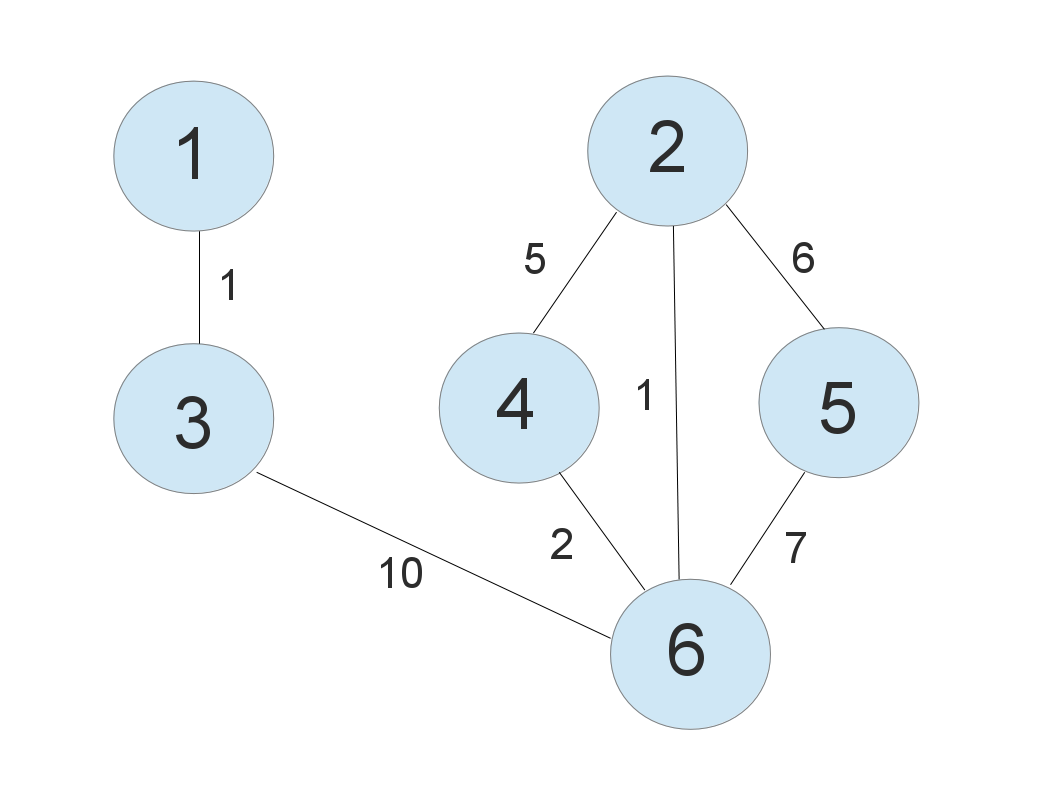
\includegraphics[scale=0.3]{ej3/imgs/graph1.png} 

\begin{figure}[H]
\center
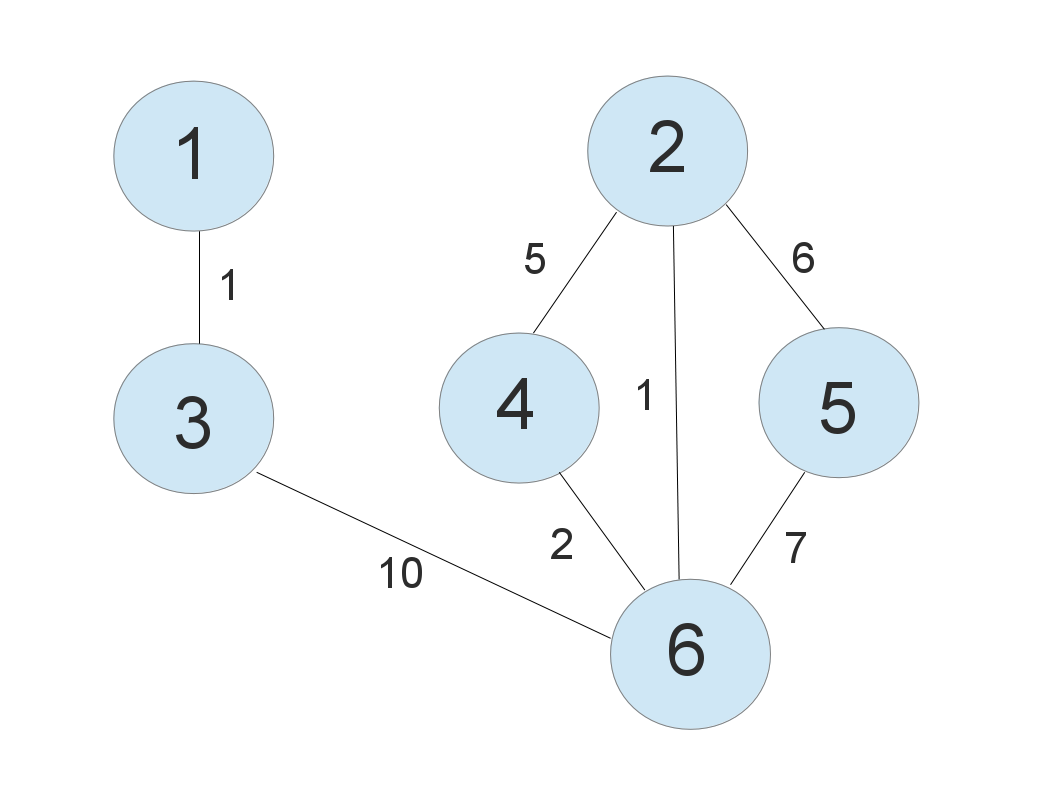
\includegraphics[scale=0.3]{ej3/imgs/graph1.png}
\caption[Long caption]{En este ejemplo disponemos de 2 fábricas y 4 clientes. Los nodos $<$ 3 representan fábricas y los $\geq \ 3$ representan clientes. El largo de cada ruta se detalla al lado de cada arista.}
\label{pic-a}
\end{figure}

Solución:

\begin{figure}[H]
\center
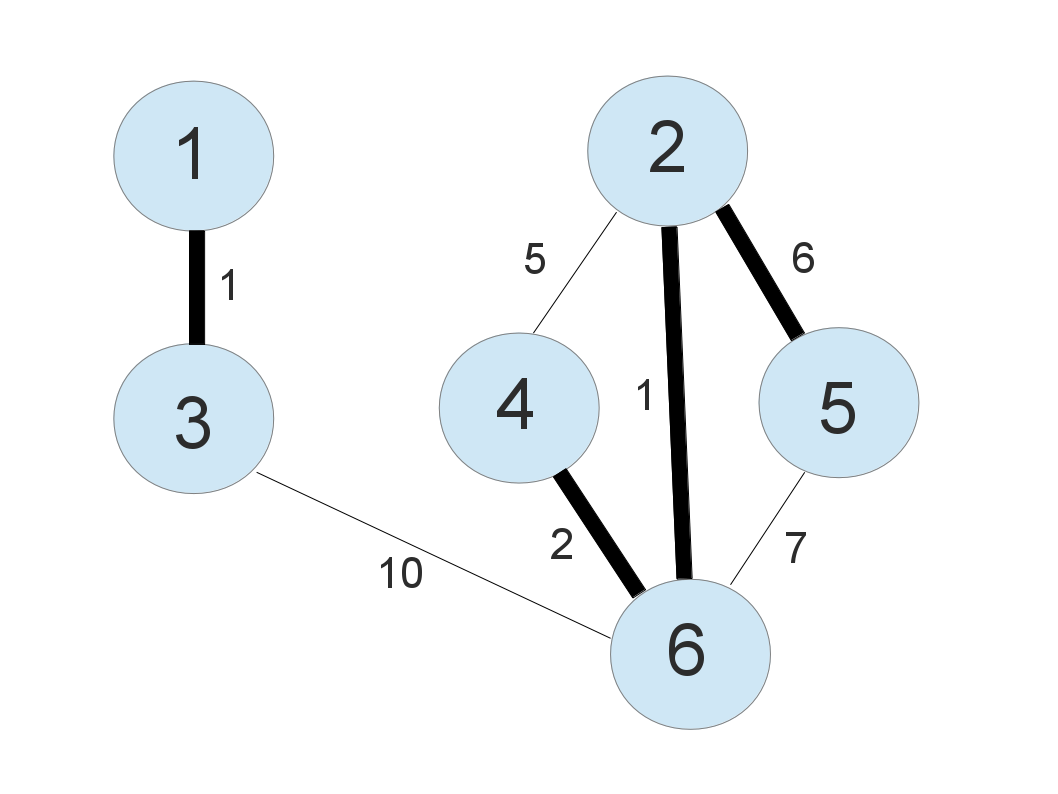
\includegraphics[scale=0.3]{ej3/imgs/graph1_sol.png}
\caption[Long caption]{Solución posible. Las rutas marcadas en negro se fortificarán.}
\label{pic-a}
\end{figure}

Cada cliente de la solución hallada es provisto por alguna de las fábricas disponibles y el costo total de inversión es minimal: 10.
